\documentclass[12pt,a4paper]{article}
%\title{Software Requirements Specification}
%\date{December 14, 2015}
%\author{Aven Bross}
\usepackage[latin1]{inputenc}
\usepackage{amsmath}
\usepackage{amsfonts}
\usepackage{amssymb}
\usepackage{amsthm}
\usepackage{enumitem}
\usepackage[english]{babel}
\usepackage{fancyhdr}
\usepackage{chngpage}
\usepackage{geometry}
\usepackage{tabularx}
\usepackage{algorithm2e}
\geometry{legalpaper, portrait, margin=1.25in}

\usepackage{tikz}

\usepackage [autostyle, english = american]{csquotes}
\MakeOuterQuote{"}

\pagenumbering{gobble}

\begin{document}

\tikzset{every loop/.style={min distance=1cm,in=-15,out=45,looseness=15}}

\begin{center}

\begin{huge}
Poh Path $3$-Coloring Algorithm for Triangulated Plane Graphs\\
\end{huge}
\hfill\\
\hfill\\
\hfill\\

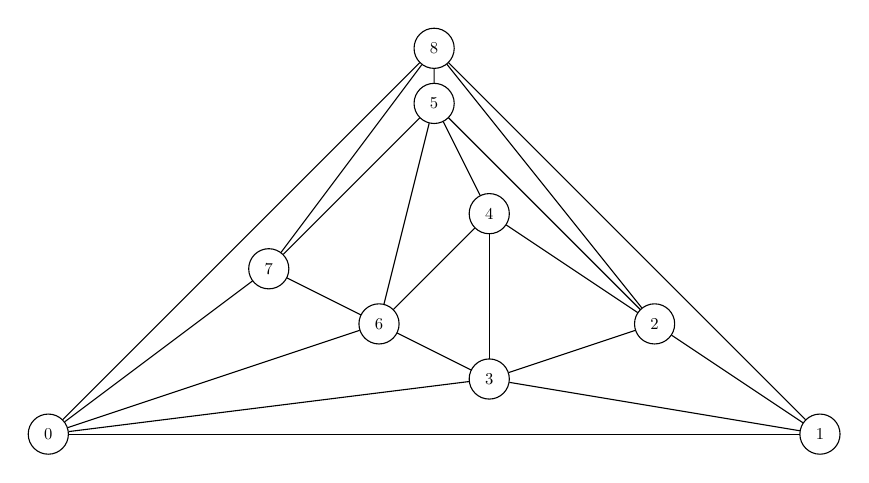
\begin{tikzpicture}[scale=.7, every node/.style={circle, draw, minimum size=8.5mm, scale=.6}]
  \node (0) at (0cm, 0cm) {$0$};
  \node (1) at (14cm, 0cm) {$1$};
  \node (2) at (11cm, 2cm) {$2$};
  \node (3) at (8cm, 1cm) {$3$};
  \node (4) at (8cm, 4cm) {$4$};
  \node (5) at (7cm, 6cm) {$5$};
  \node (6) at (6cm, 2cm) {$6$};
  \node (7) at (4cm, 3cm) {$7$};
  \node (8) at (7cm, 7cm) {$8$};
  \draw (0) -- (1);
  \draw (0) -- (8);
  \draw (8) -- (1);
  \draw (2) -- (1);
  \draw (3) -- (1);
  \draw (2) -- (8);
  \draw (3) -- (0);
  \draw (2) -- (5);
  \draw (2) -- (4);
  \draw (2) -- (3);
  \draw (3) -- (6);
  \draw (3) -- (4);
  \draw (4) -- (5);
  \draw (4) -- (6);
  \draw (5) -- (8);
  \draw (5) -- (7);
  \draw (5) -- (6);
  \draw (6) -- (0);
  \draw (6) -- (7);
  \draw (7) -- (8);
  \draw (7) -- (0);
\end{tikzpicture}\\
\hfill\\
Coloring the above maximally planar graph with the Poh path coloring algorithm.
\hfill\\
\hfill\\
\hfill\\
\hfill\\

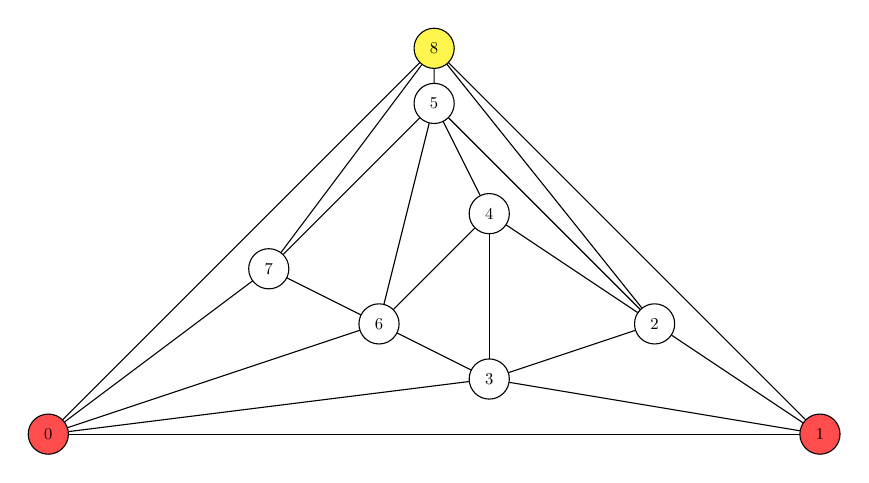
\begin{tikzpicture}[scale=.7, every node/.style={circle, draw, minimum size=8.5mm, scale=.6}]
  \node [fill=red!70] (0) at (0cm, 0cm) {$0$};
  \node [fill=red!70] (1) at (14cm, 0cm) {$1$};
  \node (2) at (11cm, 2cm) {$2$};
  \node (3) at (8cm, 1cm) {$3$};
  \node (4) at (8cm, 4cm) {$4$};
  \node (5) at (7cm, 6cm) {$5$};
  \node (6) at (6cm, 2cm) {$6$};
  \node (7) at (4cm, 3cm) {$7$};
  \node [fill=yellow!70] (8) at (7cm, 7cm) {$8$};
  \draw (0) -- (1);
  \draw (0) -- (8);
  \draw (8) -- (1);
  \draw (2) -- (1);
  \draw (3) -- (1);
  \draw (2) -- (8);
  \draw (3) -- (0);
  \draw (2) -- (5);
  \draw (2) -- (4);
  \draw (2) -- (3);
  \draw (3) -- (6);
  \draw (3) -- (4);
  \draw (4) -- (5);
  \draw (4) -- (6);
  \draw (5) -- (8);
  \draw (5) -- (7);
  \draw (5) -- (6);
  \draw (6) -- (0);
  \draw (6) -- (7);
  \draw (7) -- (8);
  \draw (7) -- (0);
\end{tikzpicture}\\
\hfill\\
1) Initial coloring of outer face.
\hfill\\
\hfill\\
\hfill\\
\hfill\\

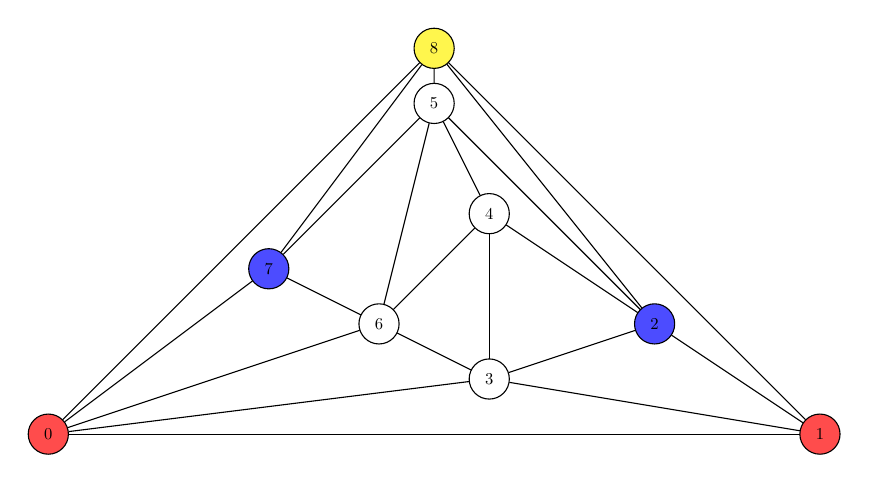
\begin{tikzpicture}[scale=.7, every node/.style={circle, draw, minimum size=8.5mm, scale=.6}]
  \node [fill=red!70] (0) at (0cm, 0cm) {$0$};
  \node [fill=red!70] (1) at (14cm, 0cm) {$1$};
  \node (2) [fill=blue!70] at (11cm, 2cm) {$2$};
  \node (3) at (8cm, 1cm) {$3$};
  \node (4) at (8cm, 4cm) {$4$};
  \node (5) at (7cm, 6cm) {$5$};
  \node (6) at (6cm, 2cm) {$6$};
  \node (7) [fill=blue!70] at (4cm, 3cm) {$7$};
  \node [fill=yellow!70] (8) at (7cm, 7cm) {$8$};
  \draw (0) -- (1);
  \draw (0) -- (8);
  \draw (8) -- (1);
  \draw (2) -- (1);
  \draw (3) -- (1);
  \draw (2) -- (8);
  \draw (3) -- (0);
  \draw (2) -- (5);
  \draw (2) -- (4);
  \draw (2) -- (3);
  \draw (3) -- (6);
  \draw (3) -- (4);
  \draw (4) -- (5);
  \draw (4) -- (6);
  \draw (5) -- (8);
  \draw (5) -- (7);
  \draw (5) -- (6);
  \draw (6) -- (0);
  \draw (6) -- (7);
  \draw (7) -- (8);
  \draw (7) -- (0);
\end{tikzpicture}\\
\hfill\\
2) Find triangulating vertices.
\hfill\\
\hfill\\
\hfill\\
\hfill\\

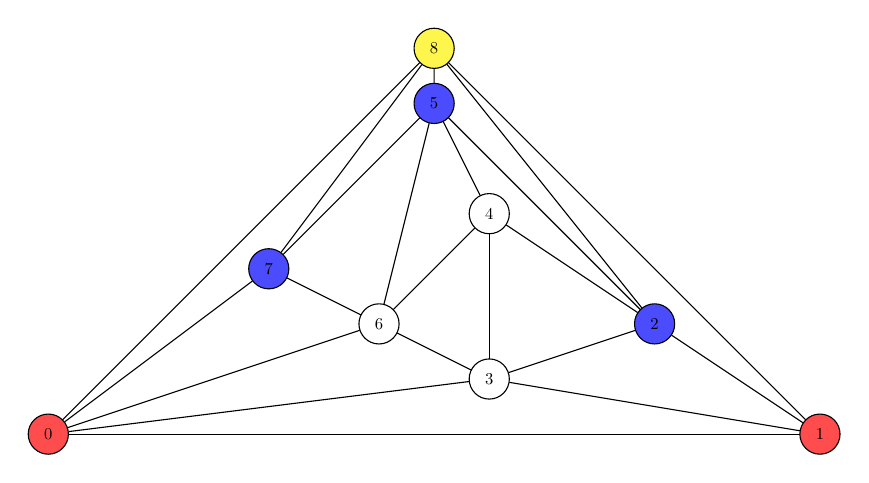
\begin{tikzpicture}[scale=.7, every node/.style={circle, draw, minimum size=8.5mm, scale=.6}]
  \node [fill=red!70] (0) at (0cm, 0cm) {$0$};
  \node [fill=red!70] (1) at (14cm, 0cm) {$1$};
  \node (2) [fill=blue!70] at (11cm, 2cm) {$2$};
  \node (3) at (8cm, 1cm) {$3$};
  \node (4) at (8cm, 4cm) {$4$};
  \node (5) [fill=blue!70] at (7cm, 6cm) {$5$};
  \node (6) at (6cm, 2cm) {$6$};
  \node (7) [fill=blue!70] at (4cm, 3cm) {$7$};
  \node [fill=yellow!70] (8) at (7cm, 7cm) {$8$};
  \draw (0) -- (1);
  \draw (0) -- (8);
  \draw (8) -- (1);
  \draw (2) -- (1);
  \draw (3) -- (1);
  \draw (2) -- (8);
  \draw (3) -- (0);
  \draw (2) -- (5);
  \draw (2) -- (4);
  \draw (2) -- (3);
  \draw (3) -- (6);
  \draw (3) -- (4);
  \draw (4) -- (5);
  \draw (4) -- (6);
  \draw (5) -- (8);
  \draw (5) -- (7);
  \draw (5) -- (6);
  \draw (6) -- (0);
  \draw (6) -- (7);
  \draw (7) -- (8);
  \draw (7) -- (0);
\end{tikzpicture}\\
\hfill\\
3) Find shortest path between triangulating vertices.
\hfill\\
\hfill\\
\hfill\\
\hfill\\

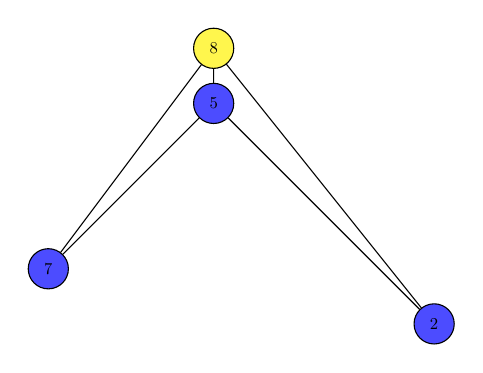
\begin{tikzpicture}[scale=.7, every node/.style={circle, draw, minimum size=8.5mm, scale=.6}]
  \node (2) [fill=blue!70] at (11cm, 2cm) {$2$};
  \node (5) [fill=blue!70] at (7cm, 6cm) {$5$};
  \node (7) [fill=blue!70] at (4cm, 3cm) {$7$};
  \node [fill=yellow!70] (8) at (7cm, 7cm) {$8$};
  \draw (2) -- (8);
  \draw (2) -- (5);
  \draw (5) -- (8);
  \draw (5) -- (7);
  \draw (7) -- (8);
\end{tikzpicture}\\
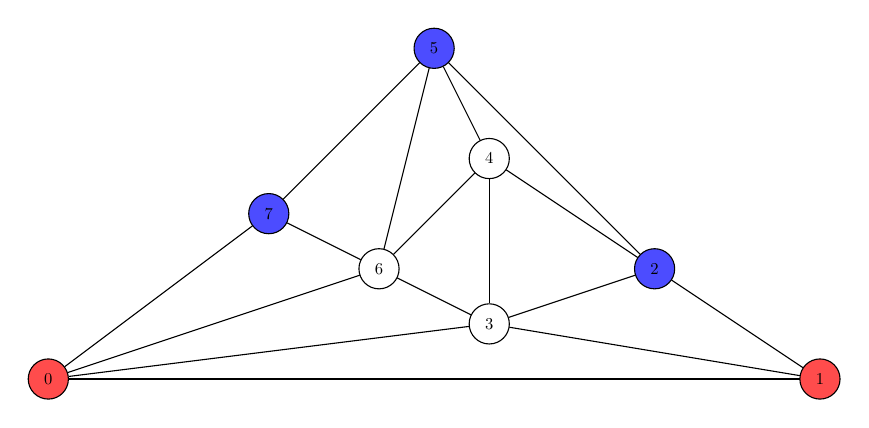
\begin{tikzpicture}[scale=.7, every node/.style={circle, draw, minimum size=8.5mm, scale=.6}]
  \node [fill=red!70] (0) at (0cm, 0cm) {$0$};
  \node [fill=red!70] (1) at (14cm, 0cm) {$1$};
  \node (2) [fill=blue!70] at (11cm, 2cm) {$2$};
  \node (3) at (8cm, 1cm) {$3$};
  \node (4) at (8cm, 4cm) {$4$};
  \node (5) [fill=blue!70] at (7cm, 6cm) {$5$};
  \node (6) at (6cm, 2cm) {$6$};
  \node (7) [fill=blue!70] at (4cm, 3cm) {$7$};
  \draw (0) -- (1);
  \draw (2) -- (1);
  \draw (3) -- (1);
  \draw (3) -- (0);
  \draw (2) -- (5);
  \draw (2) -- (4);
  \draw (2) -- (3);
  \draw (3) -- (6);
  \draw (3) -- (4);
  \draw (4) -- (5);
  \draw (4) -- (6);
  \draw (5) -- (7);
  \draw (5) -- (6);
  \draw (6) -- (0);
  \draw (6) -- (7);
  \draw (7) -- (0);
\end{tikzpicture}\\
\hfill\\
4) Split along path.
\hfill\\
\hfill\\
\hfill\\
\hfill\\

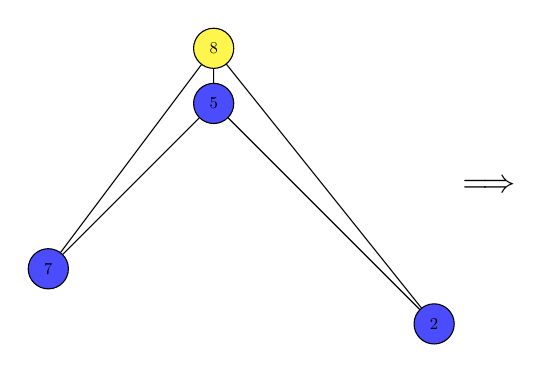
\begin{tikzpicture}[scale=.7, every node/.style={circle, draw, minimum size=8.5mm, scale=.6}]
  \node (2) [fill=blue!70] at (11cm, 2cm) {$2$};
  \node (5) [fill=blue!70] at (7cm, 6cm) {$5$};
  \node (7) [fill=blue!70] at (4cm, 3cm) {$7$};
  \node [fill=yellow!70] (8) at (7cm, 7cm) {$8$};
  \node [draw=none, scale=2] (a) at (12cm, 4.5cm) {$\Longrightarrow$};
  \draw (2) -- (8);
  \draw (2) -- (5);
  \draw (5) -- (8);
  \draw (5) -- (7);
  \draw (7) -- (8);
\end{tikzpicture}
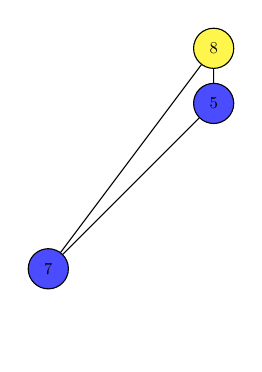
\begin{tikzpicture}[scale=.7, every node/.style={circle, draw, minimum size=8.5mm, scale=.6}]
  \node (5) [fill=blue!70] at (7cm, 6cm) {$5$};
  \node (7) [fill=blue!70] at (4cm, 3cm) {$7$};
  \node [fill=yellow!70] (8) at (7cm, 7cm) {$8$};
  \node (2) [draw=none] at (4cm, 2cm) {$$};
  \draw (5) -- (8);
  \draw (5) -- (7);
  \draw (7) -- (8);
\end{tikzpicture}
$\qquad$
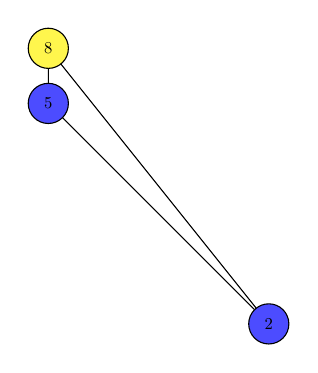
\begin{tikzpicture}[scale=.7, every node/.style={circle, draw, minimum size=8.5mm, scale=.6}]
  \node (2) [fill=blue!70] at (11cm, 2cm) {$2$};
  \node (5) [fill=blue!70] at (7cm, 6cm) {$5$};
  \node [fill=yellow!70] (8) at (7cm, 7cm) {$8$};
  \draw (2) -- (8);
  \draw (2) -- (5);
  \draw (5) -- (8);
\end{tikzpicture}\\
\hfill\\
5) Recurse on top and split on bridging edge.
\hfill\\
\hfill\\
\hfill\\
\hfill\\

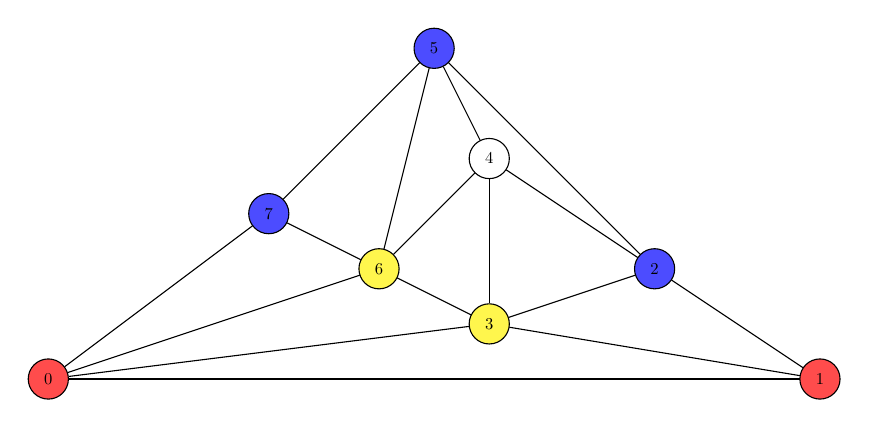
\begin{tikzpicture}[scale=.7, every node/.style={circle, draw, minimum size=8.5mm, scale=.6}]
  \node [fill=red!70] (0) at (0cm, 0cm) {$0$};
  \node [fill=red!70] (1) at (14cm, 0cm) {$1$};
  \node (2) [fill=blue!70] at (11cm, 2cm) {$2$};
  \node (3) [fill=yellow!70] at (8cm, 1cm) {$3$};
  \node (4) at (8cm, 4cm) {$4$};
  \node (5) [fill=blue!70] at (7cm, 6cm) {$5$};
  \node (6) [fill=yellow!70] at (6cm, 2cm) {$6$};
  \node (7) [fill=blue!70] at (4cm, 3cm) {$7$};
  \draw (0) -- (1);
  \draw (2) -- (1);
  \draw (3) -- (1);
  \draw (3) -- (0);
  \draw (2) -- (5);
  \draw (2) -- (4);
  \draw (2) -- (3);
  \draw (3) -- (6);
  \draw (3) -- (4);
  \draw (4) -- (5);
  \draw (4) -- (6);
  \draw (5) -- (7);
  \draw (5) -- (6);
  \draw (6) -- (0);
  \draw (6) -- (7);
  \draw (7) -- (0);
\end{tikzpicture}\\
\hfill\\
6) Recurse on bottom and find triangulation vertices.
\hfill\\
\hfill\\
\hfill\\
\hfill\\

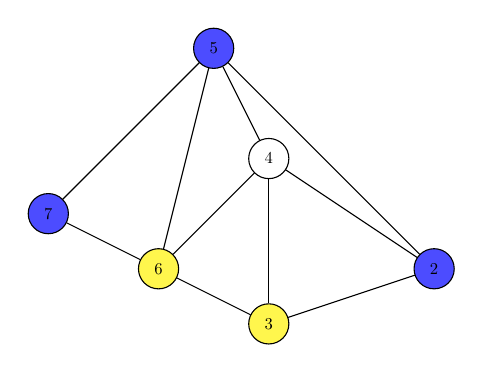
\begin{tikzpicture}[scale=.7, every node/.style={circle, draw, minimum size=8.5mm, scale=.6}]
  \node (2) [fill=blue!70] at (11cm, 2cm) {$2$};
  \node (3) [fill=yellow!70] at (8cm, 1cm) {$3$};
  \node (4) at (8cm, 4cm) {$4$};
  \node (5) [fill=blue!70] at (7cm, 6cm) {$5$};
  \node (6) [fill=yellow!70] at (6cm, 2cm) {$6$};
  \node (7) [fill=blue!70] at (4cm, 3cm) {$7$};
  \draw (2) -- (5);
  \draw (2) -- (4);
  \draw (2) -- (3);
  \draw (3) -- (6);
  \draw (3) -- (4);
  \draw (4) -- (5);
  \draw (4) -- (6);
  \draw (5) -- (7);
  \draw (5) -- (6);
  \draw (6) -- (7);
\end{tikzpicture}\\
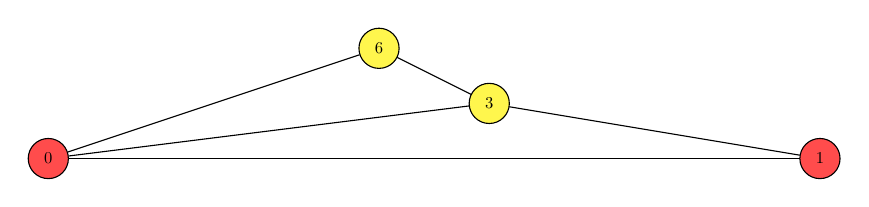
\begin{tikzpicture}[scale=.7, every node/.style={circle, draw, minimum size=8.5mm, scale=.6}]
  \node [fill=red!70] (0) at (0cm, 0cm) {$0$};
  \node [fill=red!70] (1) at (14cm, 0cm) {$1$};
  \node (3) [fill=yellow!70] at (8cm, 1cm) {$3$};
  \node (6) [fill=yellow!70] at (6cm, 2cm) {$6$};
  \draw (0) -- (1);
  \draw (3) -- (1);
  \draw (3) -- (0);
  \draw (3) -- (6);
  \draw (6) -- (0);
\end{tikzpicture}\\
\hfill\\
7) Split along path.
\hfill\\
\hfill\\
\hfill\\
\hfill\\

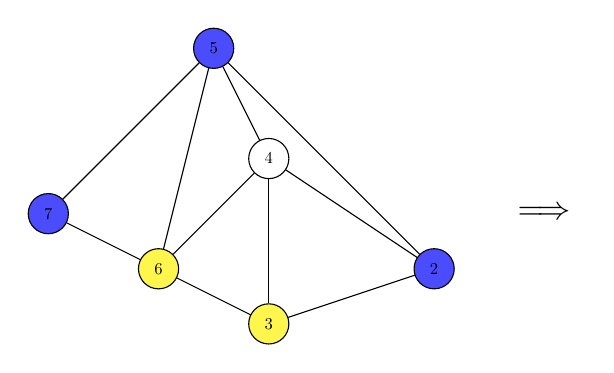
\begin{tikzpicture}[scale=.7, every node/.style={circle, draw, minimum size=8.5mm, scale=.6}]
  \node (2) [fill=blue!70] at (11cm, 2cm) {$2$};
  \node (3) [fill=yellow!70] at (8cm, 1cm) {$3$};
  \node (4) at (8cm, 4cm) {$4$};
  \node (5) [fill=blue!70] at (7cm, 6cm) {$5$};
  \node (6) [fill=yellow!70] at (6cm, 2cm) {$6$};
  \node (7) [fill=blue!70] at (4cm, 3cm) {$7$};
  \node (a) [draw=none, scale=2] at (13cm, 3cm) {$\Longrightarrow$};
  \draw (2) -- (5);
  \draw (2) -- (4);
  \draw (2) -- (3);
  \draw (3) -- (6);
  \draw (3) -- (4);
  \draw (4) -- (5);
  \draw (4) -- (6);
  \draw (5) -- (7);
  \draw (5) -- (6);
  \draw (6) -- (7);
\end{tikzpicture}
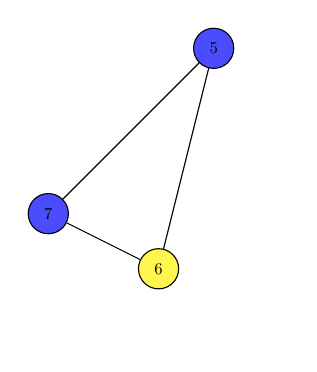
\begin{tikzpicture}[scale=.7, every node/.style={circle, draw, minimum size=8.5mm, scale=.6}]
  \node (3) [draw=none] at (8cm, 1cm) {$$};
  \node (5) [fill=blue!70] at (7cm, 6cm) {$5$};
  \node (6) [fill=yellow!70] at (6cm, 2cm) {$6$};
  \node (7) [fill=blue!70] at (4cm, 3cm) {$7$};
  \draw (5) -- (7);
  \draw (5) -- (6);
  \draw (6) -- (7);
\end{tikzpicture}
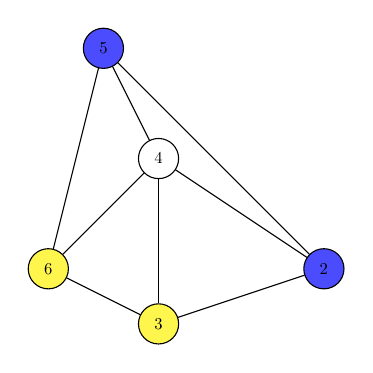
\begin{tikzpicture}[scale=.7, every node/.style={circle, draw, minimum size=8.5mm, scale=.6}]
  \node (2) [fill=blue!70] at (11cm, 2cm) {$2$};
  \node (3) [fill=yellow!70] at (8cm, 1cm) {$3$};
  \node (4) at (8cm, 4cm) {$4$};
  \node (5) [fill=blue!70] at (7cm, 6cm) {$5$};
  \node (6) [fill=yellow!70] at (6cm, 2cm) {$6$};
  \draw (2) -- (5);
  \draw (2) -- (4);
  \draw (2) -- (3);
  \draw (3) -- (6);
  \draw (3) -- (4);
  \draw (4) -- (5);
  \draw (4) -- (6);
  \draw (5) -- (6);
\end{tikzpicture}
\hfill\\
\hfill\\
8) Recurse on top and split along bridging edge.
\hfill\\
\hfill\\
\hfill\\
\hfill\\

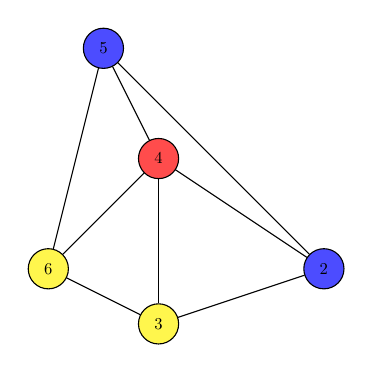
\begin{tikzpicture}[scale=.7, every node/.style={circle, draw, minimum size=8.5mm, scale=.6}]
  \node (2) [fill=blue!70] at (11cm, 2cm) {$2$};
  \node (3) [fill=yellow!70] at (8cm, 1cm) {$3$};
  \node (4) [fill=red!70] at (8cm, 4cm) {$4$};
  \node (5) [fill=blue!70] at (7cm, 6cm) {$5$};
  \node (6) [fill=yellow!70] at (6cm, 2cm) {$6$};
  \draw (2) -- (5);
  \draw (2) -- (4);
  \draw (2) -- (3);
  \draw (3) -- (6);
  \draw (3) -- (4);
  \draw (4) -- (5);
  \draw (4) -- (6);
  \draw (5) -- (6);
\end{tikzpicture}
\hfill\\
\hfill\\
9) Find triangulation vertices and splitting path.
\hfill\\
\hfill\\
\hfill\\
\hfill\\

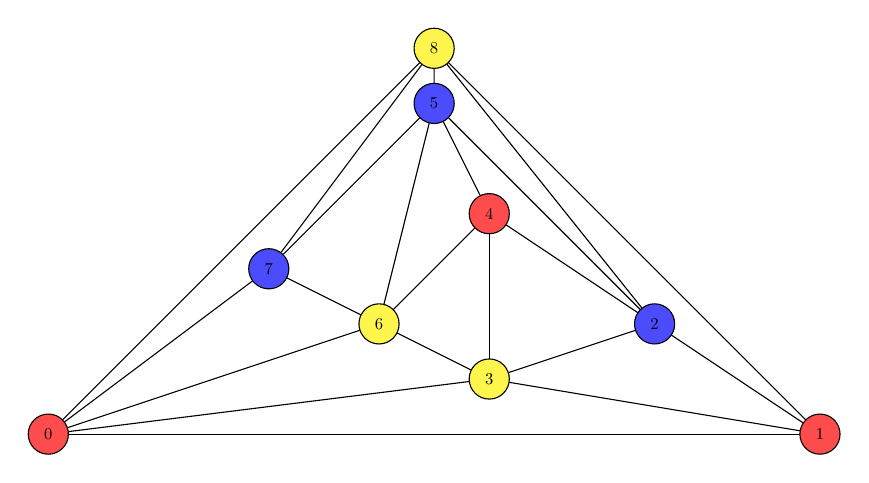
\begin{tikzpicture}[scale=.7, every node/.style={circle, draw, minimum size=8.5mm, scale=.6}]
  \node [fill=red!70] (0) at (0cm, 0cm) {$0$};
  \node [fill=red!70] (1) at (14cm, 0cm) {$1$};
  \node [fill=blue!70] (2) at (11cm, 2cm) {$2$};
  \node [fill=yellow!70] (3) at (8cm, 1cm) {$3$};
  \node [fill=red!70] (4) at (8cm, 4cm) {$4$};
  \node [fill=blue!70] (5) at (7cm, 6cm) {$5$};
  \node [fill=yellow!70] (6) at (6cm, 2cm) {$6$};
  \node [fill=blue!70] (7) at (4cm, 3cm) {$7$};
  \node [fill=yellow!70] (8) at (7cm, 7cm) {$8$};
  \draw (0) -- (1);
  \draw (0) -- (8);
  \draw (8) -- (1);
  \draw (2) -- (1);
  \draw (3) -- (1);
  \draw (2) -- (8);
  \draw (3) -- (0);
  \draw (2) -- (5);
  \draw (2) -- (4);
  \draw (2) -- (3);
  \draw (3) -- (6);
  \draw (3) -- (4);
  \draw (4) -- (5);
  \draw (4) -- (6);
  \draw (5) -- (8);
  \draw (5) -- (7);
  \draw (5) -- (6);
  \draw (6) -- (0);
  \draw (6) -- (7);
  \draw (7) -- (8);
  \draw (7) -- (0);
\end{tikzpicture}\\
\hfill\\
Done!
\end{center}

\end{document}